\chapter{Sh\"{o}wn: Adaptive Conceptual Guidance Aids Example Use}
\label{chapter:shown}
\begin{quote}
    Examples are powerful tools for creativity and can provide inspiration and structure. However, novices often don't know when to seek examples or how to apply them. 
    Showing real-time examples targeted to the current task (adaptive conceptual guidance) may help novices consider inspiration more often and better implement the ideas that examples illustrate.
    We explore this in a Wizard-of-Oz system, \textit{Sh{\"o}wn}, that presents examples based on the user's current activity while drawing a comic strip. \textit{Sh{\"o}wn}'s design is informed by interviews with novice and expert comic artists (n=18). A between-subjects experiment (n=24) found that adaptive conceptual guidance improved the clarity and uniqueness of drawings and stories compared to non-adaptive examples. Users also found the examples more useful and inspirational than those without adaptive guidance. Our results present an initial exploration of the challenges and benefits of contextually showing examples in interactive creativity tools.
\end{quote}
\section{Harnessing the Power of Examples in Creative Work}

A perennial challenge for novices is figuring out how to get started on a creative endeavor. Viewing and adapting others' work can help novices find traction in a mountain of possibility. Good examples can give inspiration, unveil new ideas, and highlight the advantages of alternative paths \cite{chan2011benefits,Siangliulue}. Examples can also help people compare and contrast different ideas across examples, drawing attention to important features (such as the composition or color scheme used by a painting) that a creator might apply to their own work \cite{alfieri2013learning,chi2012seeing,gentner2003learning,kulkarni2012early,marsh1996examples}. 

Today, with the proliferation of online communities and galleries, real examples of creative work are highly accessible.
Communities like Behance (www.behance.net) and HitRecord (www.hitrecord.org) present examples in searchable galleries that enable users to browse, modify, and implement ideas from creators with diverse backgrounds and levels of expertise, bolstering exploration and inspiration \cite{kang2018paragon,Lee2009,Lee2010}. Another strategy for supporting novices is to present examples within tools. Tools such as iMovie (www.apple.com/imovie) and Adobe Spark (www.spark.adobe.com) leverage expertise through provided templates or expert patterns. Novices in particular benefit from templates because they can shape their ideas and work to the high-level structure provided by the template \cite{Kim, kumar2011, yuan2016}.
For more procedural tasks, video tutorials serve as accessible examples that give guidance and important factual information for achieving concrete goals \cite{van2003} such as knitting a tri-colored scarf or sketching a human face. Presenting examples enables people to follow in the footsteps of others, giving a point of comparison and achievement for their own work.

\subsection{The Challenges of Applying Examples}
In order to use examples effectively, users must be able to assess the context and concept of the suggested example being presented. For example, if a novice photographer sees an example of a sunset photo with an off-center composition, they may not understand how the framing or composition affects the overall photo quality.  
Presenting examples shares similarities to search interfaces where a primary challenge is how to select and present the most relevant example or result \cite{hearst2009search,matejka2011ambient}. 
Even when examples are present and available, novices especially may not understand what examples are most relevant or how to implement the ideas within them, instead replicating surface details \cite{javadi2012impact}. Without requisite domain knowledge, discerning how to build upon examples without simply replicating them can be difficult.  

While examples can give inspiration, they can also paradoxically constrain creativity. Examples that are too semantically different from the target goal might actually be harmful for ideation \cite{chan2011benefits,chan2017semantically}.  Timing of examples also matters; examples presented too late are no more beneficial for creative outcomes than not viewing examples at all \cite{kulkarni2012early,Siangliulue}. Additionally, when given specific examples, novices tend to conform to salient surface features of examples and apply them to their own outcomes, causing potential fixation and decreasing novelty of ideas \cite{jansson1991design,kulkarni2012early,marsh1996examples,Smith1993}. Similar to work comparing experts and novices, novices tend to focus on the details of examples rather than on the underlying concepts \cite{chi1981categorization}. An important consideration for presenting examples is choosing the right examples at the right moments.

% inline websites (get rid of the https)

\subsection{Adaptive Conceptual Guidance: Examples in Context}
This chapter investigates \emph{adaptive conceptual guidance}, which presents in-situ examples and helps users apply insights from them. We show high-level domain principles at specific points in time as a user works to suggest relevant options that they may not notice or consider. In contrast to providing a library of examples or providing templates \cite{kang2018paragon,Lee2009,marks1997design,terry2002side}, this approach contextualizes examples based on the user's activity to give specific help at the right moments, which we hypothesize will aid example use and creative outcomes. 

We investigate this hypothesis through implementing a Wizard-of-Oz prototype called \emph{Sh{\"o}wn} that uses adaptive conceptual guidance to help novices explore and apply examples in the domain of comic drawing.
We choose comics as a domain because it involves multimedia storytelling and does not require special equipment, making it a useful exemplary domain for studying the challenges related to creative decision-making when multiple media (such as writing, drawing, and story pacing) are involved. 
To unearth concrete novice and expert differences for this domain, we conducted participant observations with nine expert comic artists and nine novices. We found that novices, in contrast to experts, focus on low-level detail when asked to create a comic strip and struggle to explore alternative compositions and story ideas.

We evaluated adaptive conceptual guidance in a between-subjects experiment where participants created a comic strip. This experiment ($n=24$) compared comics created by participants using one of two versions of Sh{\"o}wn:
a) a version that provided examples for users to browse on their own and b) a version that provided adaptive conceptual guidance and examples to illustrate possible ways of framing or composing comic panels. Adaptive conceptual guidance enabled participants to create comics that were rated by readers as having more unique and clear stories and drawings than comics created without adaptive guidance (Figure \ref{fig:woz}). Raters also preferred comics created with adaptive conceptual guidance overall. Participants stated in interviews that guidance inspired them to consider different ways of showing their story, lending support to the hypothesis that adaptive conceptual guidance assists exploration. Most participants without adaptive conceptual guidance either did not view the examples or did not find them useful, further supporting the hypothesis that novices need guidance for knowing how and when to implement examples to their own work. 

% To summarize, this chapter contributes the following:
% \begin{itemize}
%     \item an interview study that demonstrates how novices focus on details and struggle with exploring alternative ways to show their comic story,
%     \item a Wizard-of-Oz system that contextualizes and adaptively suggests examples and concepts at particular moments based on a user’s activity, and 
%     \item empirical evidence that adaptive conceptual guidance can help novices better utilize examples to improve their creative outcomes.
% \end{itemize}
% \section{Related Work}
\subsection{Good Feedback is Actionable, yet Rare}
Rapid iteration is critical to the success of creative projects, from essays, to visual design, to buildings \cite{Dow2010, sadler1989formative}. Receiving feedback early on is important for learners to test alternatives and course-correct \cite{Dow2010, tohidi2006getting}. Effective feedback is especially important in educational settings where novices are learning new skills and developing expertise. However, giving effective feedback is rarely taught \cite{Nicol2006}. As physical and digital classrooms increase in size, the demand for feedback outgrows the ability to adopt the ideal learning model of one-to-one feedback \cite{bloom1984}. Instead, a one-to-many approach is utilized, where an expert provides feedback for multiple learners. Although learners most value expert feedback \cite{Gielen2010, Yang2006}, the one-to-many approach is highly demanding on experts, and effective feedback for individuals becomes increasingly rare. 

In general, effective feedback is specific, actionable, and justified. Specific feedback is direct and related to a particular part of the work rather than vaguely referent \cite{Krause2017, sadler1989formative, yuan2016}. Specific positive feedback also highlights strengths of the work and provides encouragement, so the recipient can tell they are on a good path \cite{Kelley2013, Tseng2007, yuan2016}. Actionable feedback is important because it offers the learner a concrete step forward \cite{sadler1989formative, sommers1980revision, Tseng2007, yuan2016}. Simply pointing out a problem is not sufficient to help one improve \cite{Ramaprasad1983, sadler1989formative, sommers1980revision, tohidi2006getting}. Actionable feedback is often most helpful early in a project \cite{Cho2006, Tseng2007, yuan2016} because it may help people self-reflect and self-evaluate their work \cite{Gibbs}, prompting more revisions for improvement \cite{Dow2012, Topping1998}. Lastly, justification is an important characteristic of feedback \cite{Krause2017, Narciss2006, yuan2016}, but is arguably one of the hardest to understand or recognize \cite{Gielen2010}. Justified feedback contains an explanation or reason for a suggested change, which helps the learner understand why the feedback was given.

\subsection{Rubrics \& Examples Usefully Focus Feedback}
Rubrics \cite{andrade2005teaching, yuan2016} and comparative examples \cite{Krause2017} are effective in structuring feedback because they beneficially encourage attention to deep and diverse criteria. Novices otherwise tend to focus on the first thing they notice, often surface-level details \cite{Greenberg2015, hicks2016framing, Kulkarni2015, yuan2016}. Viewing examples of past designs can lead to greater creativity and insights \cite{kulkarni2012early, marsh1996examples}; thus, showing examples of good feedback may spark ideas reviewers would not have otherwise considered \cite{Greenberg2015, kulkarni2013peer, Luther2015}. Also, adaptive examples curated to match design features are more helpful than random examples in improving creative work \cite{Lee2010}. 

Rubrics and other scaffolds require significant upfront manual work by experts who must carefully design a comprehensive rubric, curate a thorough set of examples, or decide how else to structure the feedback process. This chapter investigates leveraging existing feedback to dynamically create rubric criteria. We hypothesize that showing reviewers previously-provided feedback can guide their attention to important aspects of the design. 

\subsection{Is Feedback Too Context-specific for Practical Reuse?}
Schön persuasively argues that effective feedback should be context-specific and expert-generated \cite{schon1984reflective}. He offers a vignette from architecture where the teacher suggests an alternative building to the student as an example of situated wisdom and its transfer. If Sch\"{o}n is right that this exchange requires both wisdom and context, does that mean that feedback reuse is infeasible? Within a given setting, project, or genre, common issues recur. Hewing to the principle of recognition over recall, we hypothesize that suggestions and guidance can increase novices' participation in context-specific exchanges. 

\subsection{Prior Systems \& Approaches for Scaling Feedback}
Existing approaches for scaling personalized feedback include clustering by similarity (\textit{e.g.}, for writing \cite{Brooks2014} and programming \cite{Glassman2015, Head2017}). Gradescope \cite{Gradescope} and Turnitin \cite{Turnitin} allow graders to create reusable rubric items and comments to address common issues and apply them across multiple assignments. Gradescope binds rubric items to scores, which emphasizes grades rather than improvement. 

Other methods include automating the reuse of the solutions of previous learners. These methods work best when correct and incorrect solutions are clearly distinct, such as in programming \cite{Glassman2016, Hartmann2010} and logical deductions \cite{Fast2013}. Automated methods have also found success with the formal aspects of more open-ended domains such as writing \cite{Brooks2014, Roscoe2014}.  However, assessing the quality and effectiveness of creative work – the strength of a design, the power of a poem – is intrinsically abstract and subjective and lies beyond current automated analysis techniques. Also, little automated analysis exists for media other than text. For domains like design, human-in-the-loop analysis will remain important for quite some time. 

\subsection{Automatically Detecting Feedback Characteristics}
Although feedback is often specific and contextual \cite{schon1984reflective}, general characteristics can be automatically detected and used to help reviewers improve their feedback. For example, PeerStudio \cite{Kulkarni2015} detects when comments can be improved based on the length of the comment and the number of relevant words. Data mining and natural-language processing techniques can also automatically detect whether a comment is actionable or not, and prompt the reviewer to include a solution \cite{Nguyen2016, Xiong2012}. Krause \textit{et al.} use a natural-language processing model to detect linguistic characteristics of feedback and suggest examples to reviewers to help them improve their comment \cite{Krause2017}. These methods require a reviewer to first submit their comment so it can be analyzed, and then improve their comment after submission.

\section{Interviews: Expert \& Novice Differences in Comic Drawing Process}
\label{sec:shown_ints} 

\subsection{Method: Interviewing Expert Artists \& Novices}
Differences in experts and novices have been well-studied in various domains from chess \cite{Chase1973} to physics \cite{chi1981categorization}; experts are able to contextually apply different high-level strategies to their work while novices often focus on details. We wanted to understand where novices struggle most in the domain of drawing comics to learn about the types of examples that would be most beneficial to support in an adaptive creativity support tool. 
We interviewed and observed nine expert artists and nine novices as they performed a comic-drawing task. We chose comics as a domain because most people would likely benefit from examples when engaging in the intersection of verbal and visual storytelling \cite{abel2008drawing,eisner2008comics, mccloud2006making} and because drawing comics requires only pen and paper at a minimum. 

We recruited experts from the freelance site Upwork, and novices through social media posts. Experts had formal art training and professional experience in making comic strips. We recruited novices who had a familiarity with comics, but no experience making comics and no formal education or professional experience in art. Over the course of an hour, participants drew a four-panel comic for one of three randomly given prompts: 

\begin{itemize}
\item{\textsc{Penguin}: a man befriends a penguin because of shared interests,}
\item{\textsc{Aliens}: aliens invade Earth during the 2020 global pandemic quarantine, and} \item{\textsc{Character}: a woman is upset at her date because he doesn't know who her favorite television or movie character is.} 

\end{itemize}
We asked participants to think aloud as they drew and asked questions about their process. After participants finished drawing, we asked them what they found easiest and hardest about making their comics, what the feel is the most important part of comics, and what type of help they feel would be most useful. All interviews took place on the Zoom video conferencing platform, and participants were allowed to draw digitally or use pen and paper. Experts received USD \$60 payment for their participation; novices received a \$25 gift card.

\begin{figure*}
  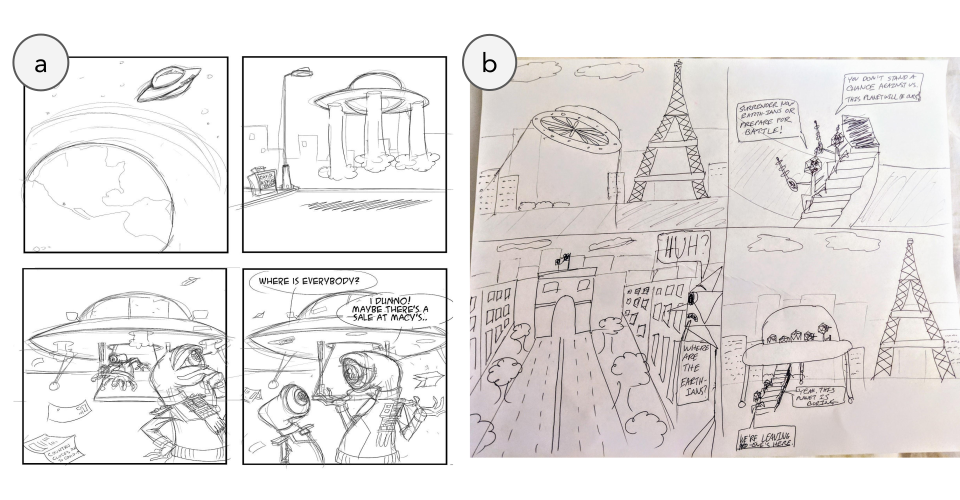
\includegraphics[width=\textwidth]{shown/figures/study1.png}
  \caption{Examples of an a) expert and b) novice comic for the \textsc{Aliens} prompt: aliens invade Earth during the 2020 global pandemic quarantine.}
  \label{fig:study1}
\end{figure*}

\subsection{Results}

\subsubsection{Experts Focus on Story \& Composition}
All nine expert artists expressed that story and composition are the most important parts of a comic: ``\textit{It’s all about composition because if you can’t understand how a comic moves, the narrative kind of decomposes}'' (Expert 4). Experts stressed that good drawing skills alone do not make a comic interesting, explaining that writing is more critical to a good comic than the fidelity of its drawings: ``\textit{I feel like the most important part is the composition of each panel because you can have great illustration..., but if the composition leads to just a random object in the background that isn’t important to the story..., the audience is going to miss something}'' (Expert 2).
Expert 8 similarly said, ``\textit{The most important thing is the writing because if you’re a good artist, but your writing stinks, you’re not going to make it. But you can have awesome writing and stick figures and make a million bucks, so to speak}.'' 

To achieve their narrative goals, experts mentioned using composition concepts and rules to help establish the flow and message of the comic. Expert 5 stated, ``\textit{There’s pretty simple rules of composition, you know, thirds, rhythm, all that stuff. They kind of help lead you to the subject’s eyelines.}'' As in prior work on expert drawing strategies \cite{Edwards1979,Poore1967}, experts drew rough sketches to rapidly outline their ideas. These quick sketches helped them evaluate their work in terms of visual concepts like composition, as well as narrative concepts like flow and pacing. For example, Expert 6 said, ``\textit{So I just plan out how I want it to look. And, you know, once you're done with something you're always like, ‘Oh, I can make that better. I can make it nicer.’ To get the general gist, we're going to see what they're doing, and etcetera.}'' Expert 1 similarly explained, ``\textit{And at this point, I'm still kind of planning stuff out. So I'm not really drawing what might be there, just kind of a reference. So I guess laying it out.}'' Three experts talked about typically creating thumbnail sketches to ideate panel compositions: ``\textit{I'll do like four or five different little sketches or thumbnails of what I think are good for the theme that I chose in my brainstorming session}'' (Expert 7). After a rough sketch, experts refine their sketch by adding in details, then move into a final inking stage to finish drawing their comic. Expert 5 said that doing a final drawing was the quickest part of the process because the idea in mind was already on paper. In general, experts spent most of their time on exploration and iteration while focusing on high-level elements like composition and flow, enabling them to finish drawing their comics quickly and simply. 

\subsubsection{Novices Focus on Details}
Verbally, novices also expressed the view that narrative arc is paramount: \textit{e.g.}, ``\textit{[The most important thing is] conveying the story I want to tell in as clear a way as possible}'' (Novice 8). Despite this, novices time allocation favored detailed drawings over composition and flow. For example, one novice drew the details of a character before deciding on story plot or composition. Another spent nearly 10 minutes drawing a person starting from the feet up in one panel, leading them to rush through subsequent panels: ``\textit{I’ve spent like 10 minutes on this, and I’m only on the feet!}'' (Novice 2)(Figure \ref{fig:novice}). In contrast to experts, novices often went straight into drawing their final comic with little conceptual planning or exploration. They were often hesitant to use sketches as exploratory tools and instead wrote out their ideas when conceptually planning their work: ``\textit{I know how to communicate my idea through words. That’s what I’m familiar with. I’m not as comfortable with drawing}'' (Novice 1). Conveying a clear story in the comic was the most important goal for all participants, but novices did not have an understanding of how to show their story visually. Figure \ref{fig:study1} shows an example of an expert and novice comic drawn for the \textsc{Aliens} story prompt. 

\begin{figure}
  \centering
  \includegraphics[width=.6\textwidth]{shown/figures/novice_detail.jpg}
  \caption{This novice from our interviews spent more than 10 minutes drawing a person from the feet up, fixating on getting the details of the character right.}
  \label{fig:novice}
\end{figure}

Interestingly, despite novices noting that narrative was the most important aspect of a comic, all novices attributed their inability to clearly tell a story to their lack of drawing skills. Novice 2 said, ``\textit{I can have an idea in my head, but actually translating it onto a comic is difficult.}'' Similarly, Novice 3 expressed that, ``\textit{I am able to visualize all of this very easily in my mind’s eye but everything else is kind of blank... It’s hard to translate that into a specific thing to draw because it’s not told to me what that might be.}'' When asked what help would be most useful for making their comic, seven of the nine novices said drawing help: ``\textit{I think generating the figures is something that could be automated, and [a computer] could have done a much better job than me}'' (Novice 7). Another expressed that drawing help would reduce tedium: ``\textit{I find drawing to be actually pretty tedious...if I could just come up with the panel and the script and give it someone or the computer that would be great}'' (Novice 6). The other two novices expressed a desire for templates or reference images to help them show their comic story.

The perceived lack of skill seemed to be a major factor in how novices chose compositions for their comic panels.
Novice 2 said, ``\textit{I'm thinking about what I want - like the image in my mind is literally what is on the square. And the way I decide what is on the square is because of my lack of drawing ability, it’s sort of like what is the simplest way that I can convey the message that I'm trying to set.}'' Exploring beyond the most achievable composition for a panel was also difficult: ``\textit{After you’ve decided on how to present the information or the previous information, and I feel like I don’t want to be repetitive..., and I didn’t know what would be the best way to draw my panel}'' (Novice 4). These observations highlighted two primary challenges for novices: 1) exploring ways to visually show their story idea, and 2) executing on that idea through drawing. Experts are able to quickly evaluate and decide upon alternatives through rough sketching whereas novices often fixate on making their single idea look an precise way. 

% As Jodi Picoult states, ``\textit{You can edit a bad page, but you can't edit a blank page}.''
\section{Guiding Drawing with Sh\"{o}wn}

Previous research in expert and novice differences find that novices focus on surface details and fixate on ideas \cite{Chase1973,chi1981categorization,jansson1991design,yuan2016}. Likewise, our observations showed that novices struggle with exploring alternative ideas and focusing excessively on details while drawing comics. We hypothesize that a system that helps novices consider and choose among options for \emph{what} to draw by presenting timely and relevant concepts and examples can help novices overcome these challenges as they work. 

Sch{\"o}n states that reflective practice is a continuous reframing and experimentation of ambiguous problems \cite{schon1984reflective}. Inspired by this articulation of reflective practice, we designed Sh{\"o}wn to explore our hypothesis. The Sh{\"o}wn Wizard-of-Oz system augments Google Jamboard, a web-based collaborative drawing tool, with two scaffolds for presenting examples: a drawing helper and adaptive conceptual guidance (Figure \ref{fig:shown}). We chose a Wizard-of-Oz method for two reasons: to study interaction recognition and contextual heuristics for presenting examples without the cost of full implementation, and to better observe how people used and applied conceptual examples \cite{walny2012understanding}. Because Google Jamboard is collaborative, the Wizard and the user can simultaneously see the other's activity by visiting the same link. This allows the Wizard to recognize the user's activity and provide assistance accordingly.

The Sh{\"o}wn interface comprises a drawing area for each comic panel, alongside selected examples. Users can flesh out panels in any order.
Following the drawing screens are a corpus of examples, adapted from McCloud's book \cite{mccloud2006making}, that show comic-specific concepts related to comic planning such as framing, transitions, and image and word combinations (Figure \ref{fig:shown}d). 
To communicate with the system, users can use voice commands or Jamboard's sticky notes feature to place notes on drawing screens. Sticky notes as an input mechanism allowed natural language text descriptions and deictic, ``put that there'' interactions \cite{engelbart1968research}.

\begin{figure}[t!]
  \includegraphics[width=\textwidth]{shown/figures/shown.png}
  \caption[Sh{\"o}wn’s interface and features.]{Sh{\"o}wn’s interface and features. a) A user wants to draw a comic panel showing a table and requests the drawing helper's assistance by typing a sticky note that says, ``Show me a table''. b) The drawing helper then provides a basic icon of the requested object in place of the sticky note request. c) As the user draws their panel, Sh{\"o}wn displays adaptive guidance on the right side of the screen in the form of a sticky note. d) The user can move to the immediate next screen to view relevant examples.}
  \label{fig:shown}
\end{figure}

\subsection{Adaptive Conceptual Guidance: Aiding Showing Relevant \\Examples at Relevant Moments}
We also found in interviews that, while novices enjoyed coming up with their own ideas and stories, they often did not know how to best visualize their ideas. To address this, Sh{\"o}wn provides adaptive conceptual guidance by first presenting high-level comic principles as a suggestion and then specific examples as the user works to inspire ideas for \emph{how} to portray their story. 
The guidance that Sh{\"o}wn currently provides is based on our interviews with experts and three concepts used by experts to decide how to convey a comic story \cite{abel2008drawing,eisner2008comics,mccloud2006making}: choice of framing, choice of moment or transition, and choice of images and words. McCloud \cite{mccloud2006making}, a comic expert and artist, writes that these concepts are part of the ``\textit{rough planning stage where a story’s events are first broken down into readable chunks}'' (\textit{pg. 11}). When presenting guidance, Sh{\"o}wn pairs an explanation of the concept with examples from McCloud’s book that show how the concept can be applied to a comic story.
(The concept of narrative flow is also mentioned in the book, but this refers to panel layout and spacing, which were not applicable to our study as we asked all participants to use the same four-panel layout.) Highlighting the concept behind examples reflects the scenario of an expert guiding a novice through a problem by explaining high-level concepts and providing specific instantiations of the concepts \cite{schon1984reflective}.

The timing of guidance is determined by the following set of recognition heuristics with three principles in mind based on prior work: examples should be related to what the user is currently doing \cite{fraser2019replay,kandel2011wrangler,kumar2011, Lee2010, ngoon2018interactive}, examples should be shown as early in the creative process as possible \cite{kulkarni2012early,Siangliulue}, and examples should be paired with an explanation of the underlying concept they illustrate \cite{javadi2012impact,ngoon2018interactive}.
\\
The three types of guidance that Sh{\"o}wn supports are:

\textbf{Consider the framing for this panel.} Framing refers to composition or use of camera angle and distance to show pertinent actions or details in the panel. This guidance is often presented on the first panel before a user begins drawing to help them get started with their comic. If the user is drawing a subsequent panel, Sh{\"o}wn presents this guidance if the panel’s framing is repeated from any previous panels (\textit{e.g.} if the user begins to use a medium shot in the second panel after using the same camera angle/shot in the first panel). 

\textbf{Consider the moment or transition between panels.} Moment or transition refer to the continuity between actions in panels and the specific moments shown as part of the story in each panel. This guidance is presented when a user moves to a new panel to help them think of transitions between panels.

\textbf{Consider the combination of images and words in this panel.} The combination of images and words refers to how words and images together can tell story more powerfully than either alone. This guidance is presented if the images between panels are similar, if a panel contains a lot of or no text or dialogue, or if the user is attempting to draw facial expressions. 

\subsection{Adaptive Conceptual Guidance in Action}
While the user is drawing their comic, the Wizard is simultaneously using the same prototype link to provide guidance to the user. As the user is drawing their comic, Sh{\"o}wn adaptively displays one of the three guidance suggestions based on the user’s current task and context. The Wizard displays guidance ambiently \cite{matejka2011ambient} on the right side of the panel page without interruption to the user via the sticky notes tool (Figure \ref{fig:shown}c). For instance, a user is drawing the same composition for two panels, in which two people are sitting at a table in the center of the page. Because of the repeated framings, the Wizard presents guidance for the user to ``\textit{consider the framing of this panel}'' in the form of a sticky note that is added to the right side of the drawing screen (Figure \ref{fig:shown}c) to provide inspiration for alternative ways of composing the panel. When the user sees the suggestion and clicks on the sticky note, the Wizard displays a specific example screen that shows examples corresponding to the concept being presented (Figure \ref{fig:shown}d). The user can then return to their drawing screen and modify their drawing if they choose. When the user moves to the next panel, the Wizard presents guidance for the user to ``\textit{consider the moment or transition between panels}'' before the user begins to draw their panel. After clicking on the sticky note, the Wizard presents examples showing different ways to use pacing in a comic narrative. Users can also proactively ask for guidance at any point by clicking the ``Show me a suggestion'' sticky note on the right side of any drawing screen. Users can also ignore guidance if they choose.

\subsection{The Drawing Helper: Freeing Focus from Detail}
In our interview study, novices experienced difficulty in executing their ideas and overly focused on details due to a lack of confidence in their drawing skills. To mitigate this and enable a larger focus on story, Sh{\"o}wn provides a drawing helper that can automatically render a basic sketch of a requested object using Google Jamboard's Autodraw feature, which presents icons that match the sketch input. We differentiate these icons from examples presented in adaptive conceptual guidance as these are basic renderings of objects rather than conceptual examples. If the options provided by Autodraw were not sufficient, the human Wizard provided a simple drawn sketch. The drawing helper was designed to draw basic objects such as a table or person rather than complex characters or scenes. For instance, a user wants to draw a comic story about two people having a dinner date. They want to draw the couple sitting at a table, but don't want to focus on the details of the table itself. The user asks the drawing helper for a table by making a sticky note with the text ``\textit{show me a table},'' and placing it in the center of the drawing screen (Figure \ref{fig:shown}a). The Wizard then produces an icon of the table in the location specified by the user (Figure \ref{fig:shown}b). Later, the user wants a drawing of a chair and this time requests an example via voice command by saying ``show me a chair.'' Sh{\"o}wn renders an icon of a chair, and the user can move the chair to where they desire on the screen. The drawing helper provides simple drawing objects so the user can then focus their attention on utilizing the conceptual examples that support the high-level narrative aspects of their comic story.
\section{Experiment}
\label{sec:shown_exp}
We wanted to test the hypothesis that a creativity support tool that offers adaptive conceptual guidance would help novices better utilize examples and improve creative outcomes than a tool that only provides non-adaptive examples.

\subsection{Method}

\subsubsection{Participants}
We recruited 24 novice participants (9 male, 15 female, median age = 22) through social media, mailing list advertisements, and the site UserTesting to evaluate our Wizard-of-Oz system. Similar to our interviews, we recruited novices that had familiarity with comics, but no formal education in art or professional experience in making comics. We also required participants to draw using a digital tablet with a stylus for ease of drawing. Half the participants were randomly assigned to the \textit{non-adaptive} condition while the other half was assigned to the \textit{adaptive} condition. The task asked participants to make a rough draft of a four-panel comic based on a randomly-assigned prompt from the interview study (\textsc{Penguin}, \textsc{Aliens}, or \textsc{Character} prompts). Four participants from each condition saw each of the three prompts. We encouraged black-and-white comics for simplicity, but using color was allowed. All one-hour sessions took place on the Zoom video conferencing platform, and participants received a USD \$25 gift card for their participation. 

\subsubsection{Procedure}
At the start of each study session, participants received a link to Sh{\"o}wn on Google Jamboard and were given a tutorial from the experimenter about Sh{\"o}wn’s features. \textit{Adaptive} condition participants created their comic in a version of Sh{\"o}wn with adaptive conceptual guidance where conceptual examples were presented selectively based on the heuristics described earlier. \textit{Non-adaptive} condition participants used an otherwise identical version of Sh{\"o}wn without adaptive conceptual guidance (the same conceptual examples were available via the example screens, but not selectively presented, similar to previous work with example galleries). All participants had access to the drawing helper because our main research question was about adaptive conceptual guidance versus non-adaptive examples. We chose to include the drawing helper for both conditions because Google Jamboard's Autodraw feature, which is the engine behind the drawing helper's icons, already exists within the tool itself.
Participants spent up to an hour drawing their comic while using a think-aloud protocol \cite{ericsson1984protocol}. At the end of the study session, participants answered post-interview questions about their process and thoughts on Sh{\"o}wn’s scaffolds. Following the study, we debriefed participants to inform them about the Wizard-of-Oz nature of the study.

\subsubsection{Measures}
We measured participants' behaviors and interactions with Sh{\"o}wn's features, such as the number of times participants used the drawing helper, viewed examples, and verbally expressed implementing concepts from the examples. We determined whether participants implemented examples either by their verbal expression of doing so or if they changed their panel after viewing examples. We also measured creative outcomes by gathering quality ratings of each comic from lay readers. We chose lay readers as raters (rather than experts) because lay readers are a large audience for comics, and because we wanted to capture overall story impact rather than technical quality, in line with the focus of both experts and novices in our interview study on narrative clarity.

Specifically, we measured comics in terms of clarity, creativity, and overall preference. In pairwise comparisons, raters from Mechanical Turk (61 unique Mechanical Turk workers) were sequentially presented with a pair of comics (two comics for the same prompt, one from each condition). For each pair, raters selected which comic they believed had more unique drawings and a more unique story (creativity), which comic had clearer drawings and a clearer story (clarity), and which comic they preferred overall. We separated drawing measures from story measures to account for potential individual differences in drawing ability. Pairing one comic from each condition for each prompt yielded 48 unique pairs (four \textit{non-adaptive} comics $\times$ four \textit{adaptive} comics $\times$ three prompts). Workers were paid USD \$1 to rate five pairs in sequence. Every pair received evaluations from at least five different raters, resulting in 306 total ratings.

\subsection{Results}

\begin{figure*}
  \includegraphics[width=\textwidth]{shown/figures/woz-results.png}
  \caption[\textit{Adaptive} condition ($n=12$) comics received significantly more preference ratings for more unique stories ($\chi^2=5.12, df=1, p<.05$), clearer drawings($\chi^2=3.91, df=1, p<.05$), clearer story ($\chi^2=5.12, df=1, p<.05$), and overall preference ($
\chi^2=7.87, df=1, p<.01$)]{\textit{Adaptive} condition ($n=12$) comics received significantly more preference ratings for more unique stories ($\chi^2=5.12, df=1, p<.05$), clearer drawings($\chi^2=3.91, df=1, p<.05$), clearer story ($\chi^2=5.12, df=1, p<.05$), and overall preference ($
\chi^2=7.87, df=1, p<.01$) than \textit{Non-adaptive} condition ($n=12$) comics. $*p<.05, **p<.01$}
  \label{fig:woz}
\end{figure*}

\subsubsection{Raters Preferred Adaptive Condition Comics Overall and for Most Other Measures}
Raters preferred \textit{adaptive} comics significantly more often than \textit{non-adaptive} comics overall (\textit{adaptive}=57.8\%, \textit{non-adaptive}=42.2\%, $
\chi^2=7.87, df=1, p<.01$) (Figure \ref{fig:woz}). In terms of clarity, raters preferred \textit{adaptive} comics more often when asked which had clearer drawings (\textit{adaptive}=55.6\%, \textit{non-adaptive}=44.4\%, $\chi^2=3.91, df=1, p<.05$) and which had clearer stories (\textit{adaptive}=56.2\%, \textit{non-adaptive}=43.8\%, $\chi^2=5.12, df=1, p<.05$). \textit{Adaptive} comics were also more often preferred when raters were asked which had more unique stories (\textit{adaptive}=56.2\%, \textit{non-adaptive}=43.8\%, $\chi^2=5.12, df=1, p<.05$). There was no significant difference in preference ratings for which comic had more unique drawings (\textit{adaptive}=53.9\%, \textit{non-adaptive}=46.1\%, $\chi^2=2.19, df=1, p=.14$). 
Figure \ref{fig:preferred} shows the most preferred comic for each measure as rated by the MTurk workers.

\subsubsection{Adaptive Conceptual Guidance Made Examples More Useful}
Sh{\"o}wn presented guidance at least three times to each \textit{adaptive} participant per session with a maximum of six times ($M=3.92$, $SD=0.90$). All \textit{adaptive} participants viewed at least one example screen at least one time while drawing, with an average of three times per session ($SD=1.13$). \textit{Adaptive} participants verbally expressed implementing concepts from examples an average of 2.17 times per session  ($SD=1.11$). In contrast, three \textit{non-adaptive} condition participants viewed examples, with an average of 0.67 examples viewed per session ($SD=1.23$)($t=4.84$, $df=21.8$, $p<.001$). 

\textit{Adaptive} participants mentioned that guidance served as inspiration, helping them think of new ways of showing their story they would not have otherwise realized. For example, P5 (\textit{adaptive}) noted, ``\textit{As I was going through I think I got into the same rhythm of what I wanted to show, and I think the [guidance] made me more cognizant of ways that I could switch things up. Like I don't think I would have thought of this last panel if I didn't get a nudge from those.}'' P16 (\textit{adaptive}), whose comic was the most preferred overall and for the most unique story, similarly stated, ``\textit{I think the [guidance] helped me consider different things. For example, for the 3rd panel, I wouldn't have considered doing a shot from the back of his head to show [the woman’s] point of view}'' (Figure \ref{fig:p16}). For the \textit{non-adaptive} participants who did view the examples, they also served as inspiration. P21 (\textit{non-adaptive}), whose comic was most preferred for having unique drawings, also cited the examples as helpful for their comic: ``\textit{[The examples] were kind of like a guide to give me a vocabulary for my intentions}.''

\begin{figure}[t]
  \hspace*{-1cm}%
  \includegraphics[width=\dimexpr\textwidth+2cm\relax]{shown/figures/preferred.png}
  \hspace*{-1cm}%
  \caption{The most preferred comics for each measure of clear drawings, unique drawings, clear story, unique story, and overall preference.}
  \label{fig:preferred}
\end{figure}

However, some \textit{non-adaptive} participants did not believe the examples were applicable. For example, P18 (\textit{non-adaptive}) stated, ``\textit{I already had an idea in mind so I didn’t really need the examples.}'' P15 (\textit{non-adaptive}) forgot the examples were available but wished he had used them after finishing his comic: ``\textit{I think I should have looked at [the examples] before I started drawing}.'' Similarly, although participants could proactively ask for guidance in the \textit{adaptive} condition, only two participants did so. One participant mentioned that he ``\textit{just wanted to see what suggestions were available}'' (P14, \textit{adaptive}). 

\subsubsection{Participants Wanted More Understandable Heuristics for Adaptive Conceptual Guidance}
The Wizard uses specific heuristics for displaying guidance. However, the heuristics Sh{\"o}wn used to decide when to show guidance, even if slightly off, could diminish the effectiveness of examples. Most felt the real-time guidance was useful: ``\textit{[The suggestions] were like a guidance for me. I don’t think I would go look at [the examples], so it was nice that they were shown throughout the drawing part}'' (P10, \textit{adaptive}). 
However, one participant wished guidance was presented at the beginning of drawing: ``\textit{I think these come a bit too late for me to use them because they're sparsed in between while I'm drawing. For example, the perspective one, I thought `oh, I should've used this earlier,' but the information just came a bit too late for me to use}'' (P6, \textit{adaptive}). 
This suggests that guidance heuristics should not be ``one-size-fits-all'' but rather allow users to adjust them based on perceived usefulness.

Some \textit{adaptive} participants also thought the timing and reasoning for presenting certain guidance was opaque. 
They wanted to know more about why particular advice was being given at a particular moment. P24 (\textit{adaptive}) stated, ``\textit{The suggestions were helpful, but it wasn't clear why that suggestion was being given. Like for the transition one, it could be that my transition isn't the best one I could use for my viewer or it could just be helping me get started so it wasn't clear why it was giving me those suggestions}.''
While adaptive conceptual guidance helped participants better understand examples, clarity around what the system is responding to would help users decide between many possible valid uses of those examples.

\begin{figure}[b!]
  \includegraphics[width=\textwidth]{shown/figures/p16.png}
  \caption{a) This comic was created using Sh{\"o}wn's adaptive conceptual guidance. b) The participant cited that seeing a relevant example inspired the composition of the third panel of the comic.}
  \label{fig:p16}
\end{figure}

\subsubsection{The Drawing Helper Shifted Focus from Details to Story}
We tracked user interactions with the drawing helper to understand how people used this feature and how it possibly interacted with example use. Participants in both conditions used the drawing helper frequently, with an average of 4.67 times ($SD=2.87$) per session for \textit{adaptive} participants and 5.67 times ($SD=4.68$) for \textit{non-adaptive} participants ($t=-0.63$, $df=18.3$, $p=.54$). In some cases, the drawing helper made drawing objects---particularly repeated objects---less tedious. For example, P24 (\textit{adaptive}) used the drawing helper to draw a phone screen that would be consistent across all panels. P11 (\textit{non-adaptive}) felt the drawing helper did indeed help him focus less on details: ``\textit{I thought [the drawing helper] was really cool, especially for like tables or chairs or to hash out the overall setting so you can just focus on the other stuff.}'' P21 (\textit{non-adaptive}) thought the drawing helper was useful for showing her intended vision: ``\textit{I could just tell [the drawing helper] my vision, and it would bring up things that are relevant}.'' 
Our findings suggest that the concreteness provided by tools like the drawing helper may complement the efficacy of strategies like adaptive conceptual guidance. 

However, a few participants felt limited in their creativity with the drawing helper. One participant noted an over-reliance on the drawing helper rather than sketching, stating, ``\textit{I kinda became too dependent on [the drawing helper]. Normally, I would just draw it out quickly, but I want to see what the system can do...With the tool, I think if the system can do this for me, and it's perfect the first time, I try to see how I can fit my idea to what the system can do}'' (P15, \textit{non-adaptive}). 
Another participant felt that the simplicity of the drawing helper's sketches did not allow them to completely show their vision: ``\textit{It was pretty limited in what it could show. Like I couldn't do perspectives or angles with the basic icons I was given}'' (P12, \textit{adaptive}). 
These observations corroborate the fact that we found no significant difference in visual creativity across the two conditions ($\chi^2=2.20, df=1, p=.14$).
Three participants did not use the drawing helper or only used it once because, as one participant stated, ``\textit{It might have been more helpful if I was drawing something more complex, but it was just easier to draw it on my own}'' (P13, \textit{non-adaptive}). 
\section{Discussion \& Future Work}
This chapter investigated whether providing adaptive conceptual guidance aids example use more effectively than non-adaptive examples through a Wizard-of-Oz prototype and empirical study. We next discuss implications of our findings for future creativity support tools and generalization to other domains. 

\subsection{System-Directed Versus User-Directed Creativity Support}
In our experiment, we observed that novices in both conditions rarely sought examples without being prompted, perhaps because they were unaware of needing help or did not know what help they needed. Only two \textit{adaptive} condition participants proactively asked for guidance, and only three \textit{non-adaptive} condition participants viewed the examples gallery on their own. While exploring alternatives is a useful problem-solving strategy, meaningfully evaluating them requires expertise and the comparison induces a hefty cognitive load \cite{tuovinen1999comparison}. In line with prior work \cite{bilalic2008good, Graesser1994,Siangliulue}, this suggests that timing is relevant to giving the most appropriate help as novices may not know what type of help is most helpful and when. By incorporating concepts with examples, we found that Sh{\"o}wn's real-time adaptive conceptual guidance helped to expand participants' field-of-view to concepts they would not have known to explore on their own. Such proactive system-directed approaches seem to benefit open-ended creative problems (like figuring out how to draw a comic story) because they help users explore beyond known possibilities.

Similar to other systems that present galleries of examples to provide broad inspiration \cite{kang2018paragon,Lee2009,marks1997design}, Sh{\"o}wn provides high-level examples meant for conceptual exploration rather than examples that are particular to the user's specific work. For example, if a user wants to draw two people talking, Sh{\"o}wn presents general examples of different panel framings or combinations of text and images rather than specific instances of two people talking in a panel. These context-agnostic examples are framed as considerations (rather than statements that impose specific approaches as the ``correct'' ones). This open-ended approach is analogous to human tutoring, where less didactic interactions allow the learner to form their own explanations and hypotheses in evaluating ideas \cite{Chi2010}. 
In addition, recommending guidance in-situ allowed participants to better understand the relevance of guidance and evaluate examples in context \cite{schon1984reflective}. One participant explicitly mentioned that showing guidance in the moment while drawing encouraged them to view the examples when they would not have otherwise. Participants cited that even if they did not change their initial idea, the provided examples served as inspiration or as a way to help them explain their choices. In these instances adaptive conceptual guidance seemed to serve as a nudge for users to consider different options or evaluate their own decisions. 

In contrast, user-directed approaches (such as query-based systems and other help-seeking tools \cite{fraser2019replay,Huang2019, Satyanarayan2014}) seem to work best when the user has a concrete idea they want to execute. We saw this with how participants made use of Sh{\"o}wn's drawing helper, which produced basic icons to quickly visualize ideas based on a user's request. Some used voice commands to direct the drawing helper to provide images. However, the drawing helper had its limits: it could not generate drawings in response to complex, ambiguous requests. For example, P15 (\textit{non-adaptive}) asked the drawing helper to lay out an entire panel: ``\textit{Show me a man holding a phone with a dating app on it and lists for interests.}’’ 
This participant attempted to shape their ideas around what the drawing helper could generate, rather than using it to show their own ideas. This reflects how novices may form an over-reliance on help-tools or conform to salient features rather than high-level considerations \cite{jansson1991design,javadi2012impact,marsh1996examples,Smith1993}. Our findings with Sh{\"o}wn suggest that user-directed guidance works best for small and concrete tasks where the user already has an idea in mind.

Both system-directed and user-directed guidance can support the creative process in complementary ways. Context-agnostic conceptual aid allows for the ambiguity of exploration while specific user-directed guidance can give a concrete direction towards accomplishing goals. In many ways, using examples as guidance is similar to coaching or tutoring, where a coach or tutor gives both open-ended hints or suggestions and concrete examples depending on a person's progress. Sh{\"o}wn provides a demonstration of using context from user actions to leverage such guidance for creative work. Future research could further examine how computational systems can provide more adaptive coaching or tutoring for creative endeavors.

% limitations of current study
\subsection{Designing Adaptive Conceptual Guidance Systems: Limitations \& Opportunities}
We found two areas where adaptive conceptual guidance could be improved. The first is in determining the timing of guidance. One participant felt that guidance was presented too late and would be more helpful or more relevant earlier. While guidance was shown adaptively, the heuristics for determining when to show certain concepts and examples were static for each participant, which is both a limitation of the Wizard-of-Oz implementation as well as potential technical implementations. One open question is how to better anticipate when to provide guidance when even the user does not know when to ask for help. Potential effective timing mechanisms might be measuring how long a user is idle \cite{chan2018best,Siangliulue} or taking a mixed-initiative approach in incorporating user input, such as refining or pruning suggestions \cite{kandel2011wrangler} to determine the best moments to present examples. 

The second area of improvement is providing transparency around why guidance was being given. Three participants wanted further explanation for why certain pieces of guidance were being shown at specific times. One participant asked the experimenter whether the system presented guidance randomly or not. Another thought the presentation of guidance meant the system did not ``like'' their current drawing. This sentiment reflects prior work showing that people prefer explainable and transparent interactions with AI systems so they not only understand what help is being given but also why \cite{Amershi,Heer2019,Oh2018}. One possibility is to display guidance alongside interactive checkboxes or dynamic rubrics to help users understand how to better situate guidance within the user’s context \cite{Bharadwaj,ngoon2018interactive}.

We also found potential in improving user-directed support. While participants did not often explicitly seek out examples while working on their comics, many participants in both our interviews and experiment asked ideation questions aloud such as ``\textit{How do I show this place is empty?}'' or ``\textit{How do I show that this character is angry?}'' as part of the think-aloud protocol. These questions could serve as queries to indicate user intent and aid in tailoring the type of examples shown. During exploratory tasks like brainstorming ideas or deliberating ways to translate an idea visually, users may have more of these open-ended queries in mind rather than concrete goals. Tools that adaptively display help for just-in-time learning as well as incorporate contextual search mechanisms like natural language and deictic instructions may be useful ways of enabling user-directed conceptual support \cite{fraser2020remap, Graesser2001, laput2013pixeltone, Yoon}. 

%limitations of system design
As a Wizard-of-Oz prototype, Sh{\"o}wn utilizes a human Wizard to use a user's actions as heuristics to determine what conceptual guidance to provide. Some of the heuristics were based simply on starting on new panels (\textit{i.e.} the Wizard shows the guidance to consider moments or transitions when the user moves on to a new panel). Other heuristics were based on capturing the user's past and current actions (\textit{i.e.} the Wizard presents guidance on images and words if the panel contained too much or too little text). Existing tools already use sketch-based actions as context such as Procreate's Quick Shape tool\footnote{https://procreate.art/handbook/procreate/guides/quickshape//} to automatically complete shapes or straighten a user's lines or Google Jamboard's Autodraw tool that uses object recognition to infer what icons to suggest to the user. Co-creative intelligent agents can also use object and line recognition to improvise collaborative drawing \cite{Davis2016}. Our Wizard-of-Oz evaluation shows how adaptive systems might use visual, sketch-based context to provide conceptual guidance beyond automated drawing help or example galleries. Open remaining questions are how systems might be trained to learn such context as well as what types of context and concepts are most appropriate for adaptive and automated assistance beyond sketching.

One limitation of Sh{\"o}wn was that the example screens were separate from the drawing screens, requiring users to switch between drawing and example screens in order to view them. Tools incorporating adaptive conceptual guidance or examples presentation should consider more ambient displays that show examples without requiring the user to change the context of their work. Because of the remote nature of the study, one limitation was that we could not control for the screen size participants used. This may have affected drawing ability, though this limitation may have been mitigated since all participants used a stylus and had the drawing helper available.

Tools that help novices overcome skill barriers to execute their creative goals are powerful, but without seeing potential alternatives and possibilities, novices remain bounded by their limited conceptual expertise. Sh{\"o}wn evaluates simple recognition heuristics through a Wizard-of-Oz implementation to contextually present concepts and examples for better exploration and execution. Future work could examine feasibility and implementation of such heuristics for creativity systems across domains. We find that combining user-led support for concrete queries and adaptive support for open-ended exploration of alternatives helps novices better understand and utilize alternatives for their own work. An interleaving of system-led support and user-led agency is a promising direction for the development and evaluation of future creative tools \cite{Heer2019}. We provide a demonstration of this direction that can apply to creative endeavors across domains.

\subsubsection{Summary}
% do this for all chapters
We present Sh{\"o}wn, a Wizard-of-Oz system that provides adaptive conceptual guidance by suggesting relevant concepts and examples for a user to explore based on their current task. We hypothesized that adaptive conceptual guidance would guide the application of examples and improve creative work more than simply providing static examples alone. Through interviews and a between-subjects experiment in the domain of comics, we found that adaptive conceptual guidance led to comics with more unique and clear stories and clearer drawings. Users also found adaptive conceptual guidance to be timely and useful for inspiration while users without guidance did not find the examples as relevant and were less likely to take advantage of them. We argue for tools that help novices explore ideas by providing the right kinds of assistance in the right situations. In this way, we may better expand novices' vantage points to explore concepts more broadly and improve creative work. This chapter provides a direction for the future of adaptive creativity support tools and presentation of examples.

\subsubsection{Acknowledgements}
We thank the novice and expert comic artists for participating in interviews and our experiment participants for their time and efforts. This research was funded in part by Adobe Research.

This chapter, in part, includes  portions of material as it appears in \textit{Sh\"{o}wn: Adaptive Conceptual Guidance Aids Example Use in Creative Tasks} by Tricia  J. Ngoon, Joy O. Kim, and Scott Klemmer in the Proceedings of the 2021 ACM Conference on Designing Interactive Systems (DIS '21). The dissertation author was the primary investigator and author of this paper.